\section{错误检查API详解}

在深入探讨使用 Nsight Compute 工具分析 CUDA 应用之前，需要强调 CUDA 函数中错误检查的重要性。用一个例子来说明这一点。在进行性能分析之前，确保 CUDA 函数运行流畅且准确至关重要。在前文中提到过一个问题，即应用程序编译时没有错误，然而该应用程序却无法正确执行。经过调查，定位到了一个故障的 \texttt{malloc} 函数，原因是用于分配所需存储或所需空间的 RAM 不足。这类错误在编译期间无法检测到，在运行时也可能不会表现为可读的错误。这凸显了为所有 CUDA 函数使用错误检查的必要性。

\subsection{内存不足问题分析}

这大致可以分为两类：同步错误检查和异步错误检查。CUDA 提供了几种机制来检查其操作或函数的成功与失败。从第一类开始：同步错误检查。在 CUDA 中，像内存分配这样的操作是同步的，这意味着这些操作会阻塞主机代码的执行，直到设备完成操作。大多数 CUDA Runtime API 函数都会返回一个错误代码，这使得错误处理更加直接，因为错误会在操作完成后立即报告。可以通过检查这个错误代码来确定是否发生了错误。

现在打开向量加法代码来做一些错误检查测试。这是在添加任何错误检查指令之前，是之前章节的向量加法应用程序。首先需要测试这个应用程序是否工作正常。打开终端，列出第四节文件夹中的所有文件。如所示，有三个文件，而本章将重点关注第 2 个 \texttt{02\_enhanced\_vector.cu}。需要编译和运行，检查编译和执行步骤中是否有任何错误。从编辑器中可以看到，打开的是同一个文件。正如之前讨论的，正在使用 NVCC 编译器。\texttt{nvcc -o} 这是可执行文件的名称。以 CUDA 文件结束命令，编译时没有出现任何错误。现在运行应用程序，执行也没有任何问题。

回到这里，把这个值，也就是 32 替换成一个更大的值，$1024 \times 25$。增加每个向量中元素总数的原因是为了增加每个向量所需的总存储量，从而在给这个应用程序分配所需空间时制造一个问题。一旦出现问题，就需要通过错误检查来确切地知道问题是什么。在那之前先简化一下，把 20 这个乘数去掉。在编译和运行应用程序之前，用任务管理器检查一下电脑资源。右键点击，然后选择任务管理器。选择性能选项卡，它显示了电脑中的所有资源。从 CPU 开始到 GPU 结束，需要关注的是内存和 GPU。

原因是关注内存，因为这里有三条指令要在 RAM 中分配空间，而 RAM 在这里由内存选项卡表示。同时使用 \texttt{cudaMalloc} 函数在 GPU 中分配空间，这就是关注 GPU 的原因。

可以注意到 GPU 现在使用了大约 48\% 的资源，内存使用了 2.5 GB。也可以从图表检查这个值。具体来说关注的是专用 GPU 内存，专用 GPU 内存指的是 GPU 内部真实或实际的内存。这是因为录制程序在运行，最后一个选项卡说明这个录制程序使用了硬件加速，硬件加速指的就是 GPU 本身。需要从这里这些步骤查看 GPU 和内存。

需要计算每个向量所需的总存储量。这里就是结果，这个数字代表了每个向量中的元素总数。复制这个数字，然后写下结果代表了每个向量中的元素数量。有三个向量，那么现在需要做的是乘以 4。为什么需要乘以 4 呢？因为应该熟悉 C 语言，在 C 语言中整数值使用四字节的存储空间，因为这些元素中的每一个都包含一个整数值。需要乘以 4 来得到每个向量所需的总字节数。但现在想以 GB 为单位计算，而不是字节。然后再除一次转换成 MB，除以 1024 转换成 KB。再进行一次转换变成 GB。如所示，每个向量将使用 4 GB 存储空间。因为有三个向量，所以将使用 12 GB。现在需要再次检查资源，GPU 现在使用了 2.5 GB，当运行这个正常的应用程序时，这个值应该从 2.5 增加到大约 14 或 15 GB。

来编译。编译时出现了一些警告，需要处理警告，因为它可能在运行时、在执行时造成问题。这不是编译时的问题。现在可以执行，编译已经完成了，但在执行时应用程序可能工作也可能无法正常工作。先关注第一个问题。它指出问题从这里这部分开始。如前所述，第十七行有个问题。读一下警告本身，它说整数转换导致截断。回到应用程序，每当看到截断部分，就应该知道这个值太大了，无法存储在分配的空间里。第十七行有一个整数值，叫做 \texttt{size}，这个变量应该存储乘以 4 字节之后的结果。取 \texttt{size}，它代表这个数字，然后乘以四字节，结果将存储在这个变量中。这里的结果太大了，无法只存储在四字节中，需要超过四字节。这就是为什么需要写 \texttt{long}，而不是 \texttt{int}。然后编译，如所示，现在没有问题或警告了，然后运行。当代码应用程序正在执行时，可以检查专用 GPU 内存，它正从 2.5 增长到 15，大约 14.7 左右，GPU 内存会出现一个峰值。

\subsection{同步错误检查实现}

现在没有问题，想把应用程序所需的空间增加到一个很大的值。可能会想错误检查在哪里？大到无法装入专用 GPU 内存，甚至共享 GPU 内存。因为如果使用例如 30 GB，那么将用掉全部 24 GB 的专用内存和 6 GB 的共享内存。想增加更多，把这个值乘以 20。如果把这个值乘以 20，那么每个向量需要 80 GB。需要三个向量乘以 80 GB，这个值将大到无法放入 CPU 的 RAM 内存，甚至 GPU 内存。现在编译看看一些其他的警告。如所示，有更多警告。从第十七行开始还是同一行。因为这里的乘法不能以这种方式进行，所有这些值 1024 都是整数。但当乘以另一个 20 时，这个值将无法装入一个整数。也许 \texttt{long} 可以，\texttt{long} 足够了，但它不足以进行乘法运算本身。需要做的是复制这部分，并定义一个空间足够的变量。写 \texttt{long}，但因为 \texttt{long} 可能还不够，所以再写一个 \texttt{long}，以确保分配超过八字节。然后写等于，加上 \texttt{LL}。因为如果去掉这个 \texttt{LL}，那么就是在整数乘整数乘整数，结果应该是 \texttt{long}。这里的 \texttt{L} 指的是需要对 \texttt{long} 值进行乘法，而不是整数。但如果乘两个值，在最终值存储到这个 \texttt{size} 之前，它不足以存储在整数值中。这就是为什么如果看警告，会在其他指令上也有警告。比如第 28 行，看 for 循环，不能在这里乘这些值，因为它们现在被定义为整数。当写 \texttt{LL} 时，意味着是在乘 \texttt{long} 值，而不是整数值。然后编译并运行。

如所示，遇到了段错误。在这种情况下，知道问题所在，这个应用程序需要的空间超过了 CPU 的 RAM 和 GPU 专用内存的可用空间。但如果有一个应用程序在输出中给出了段错误，但不知道所需空间，这就是为什么需要错误检查。需要为这三个函数，也就是 \texttt{cudaMalloc} 内存分配函数添加一些错误检查。复制指令，为这三个函数放在这里。顺便说一下，需要对 \texttt{cudaMemcpy}、\texttt{cudaEventRecord}、核函数启动等做同样的事情，这里只是把这些作为例子。这只是错误对象的声明，这个对象将用于存储每个 CUDA 函数的错误。这就是为什么这个变量或对象的类型是 \texttt{cudaError\_t}，这是 CUDA 编程中的另一种结构。需要再次写上 \texttt{error =}。如前所述，每个 CUDA 函数都会提供一个错误。这个错误随后可以被检查，以确切地知道执行这个函数的问题是什么。取这个函数的输出，并将其存储在错误对象中，然后测试这个错误是否不是 \texttt{cudaSuccess}。如果不是成功，那么就有问题。需要打印这个错误。如所示，使用了 \texttt{fprintf}，但这里的错误值不是字符串值，它更像是 ID 号之类的东西。使用另一个 CUDA API 函数叫做 \texttt{cudaGetErrorString}，它接收错误 ID 并返回对应于该 ID 的字符串。这就是为什么对所有 CUDA 函数重复相同操作，并且应该对此应用程序中的其他 CUDA 函数做同样的事。

现在保存、编译和运行。同样的问题，没有从添加到应用程序的错误检查指令中得到任何指示。原因是如果在为 GPU 内存分配之前，先为主机内存分配了空间——\texttt{malloc} 和 \texttt{cudaMalloc}——输出中的段错误出现在 \texttt{malloc} 这里，而不是 \texttt{cudaMalloc}。而且没有为 \texttt{malloc} 做错误检查。需要把这些指令向下移动。现在在为 CPU 或主机的 RAM 分配空间之前，先在 GPU 中分配空间。在这种情况下，如果 \texttt{cudaMalloc} 无法在 GPU 中分配所需空间，应该能看到错误检查的输出。

编译并运行，在运行时看看 GPU 资源会发生什么。如所示，可以检查专用值。因为需要 80 GB，编译器现在正尝试分配全部的 24 GB 专用 GPU 内存，然后尝试增加共享 GPU 内存。编译器正尝试分配第一个向量的空间。但这两者都不够，所以会看到一些峰值，它尝试然后失败，如此反复。最终编译器会说"无法为第一个向量分配空间"，它会为第二个向量 B 和第三个向量 C 做同样的事。从这部分可以看到，"未能分配设备内存不足"，这是这条指令的结果。分配内存失败原因就是内存不足。一旦完成了 GPU 的分配，无论是成功还是失败，将使用这些指令为主机端分配空间。没有足够的空间来分配所需的存储，这些指令也应该会失败，这就是为什么也有一个段错误。但在尝试先在 GPU 中分配之后，这就是它的重要性。这就是错误检查在 CUDA 应用程序中的使用方式，它给出一些指示，确切地指出问题在哪里。特别是如果有一个由他人设计的应用程序，而正试图开发或增强它，错误检查就是这样工作的。

回顾本章开头提到的内容，错误检查有两类：同步和异步错误检查。对于同步错误检查，GPU 任务、GPU 函数或 GPU 操作会阻塞主机执行任何其他指令，直到 GPU 任务完成其执行。它将在这里被阻塞，直到 \texttt{cudaMalloc} 完成其执行。例如，如果编译器执行到这里的第 27 行，那么它将停在这里。在执行中编译器将尝试为向量 A 分配空间，但它不会在完成向量 A 的分配之前尝试为向量 B 分配。完成向量 A 的分配，然后进入向量 B 的下一步，无论失败还是成功都没问题。一旦完成向量 B 进入第三步，以此类推。正如所示，现在正尝试为向量 B 分配。完成了向量 A 的步骤，它失败了，但没问题。这就是同步操作的含义。这就是为同步操作使用错误检查的方式：一个错误对象使用这条指令，然后读取同步函数的输出，然后检查该错误是成功还是失败。如果操作失败，那么需要打印错误。

\subsection{异步错误检查}

\begin{figure}
    \centering
    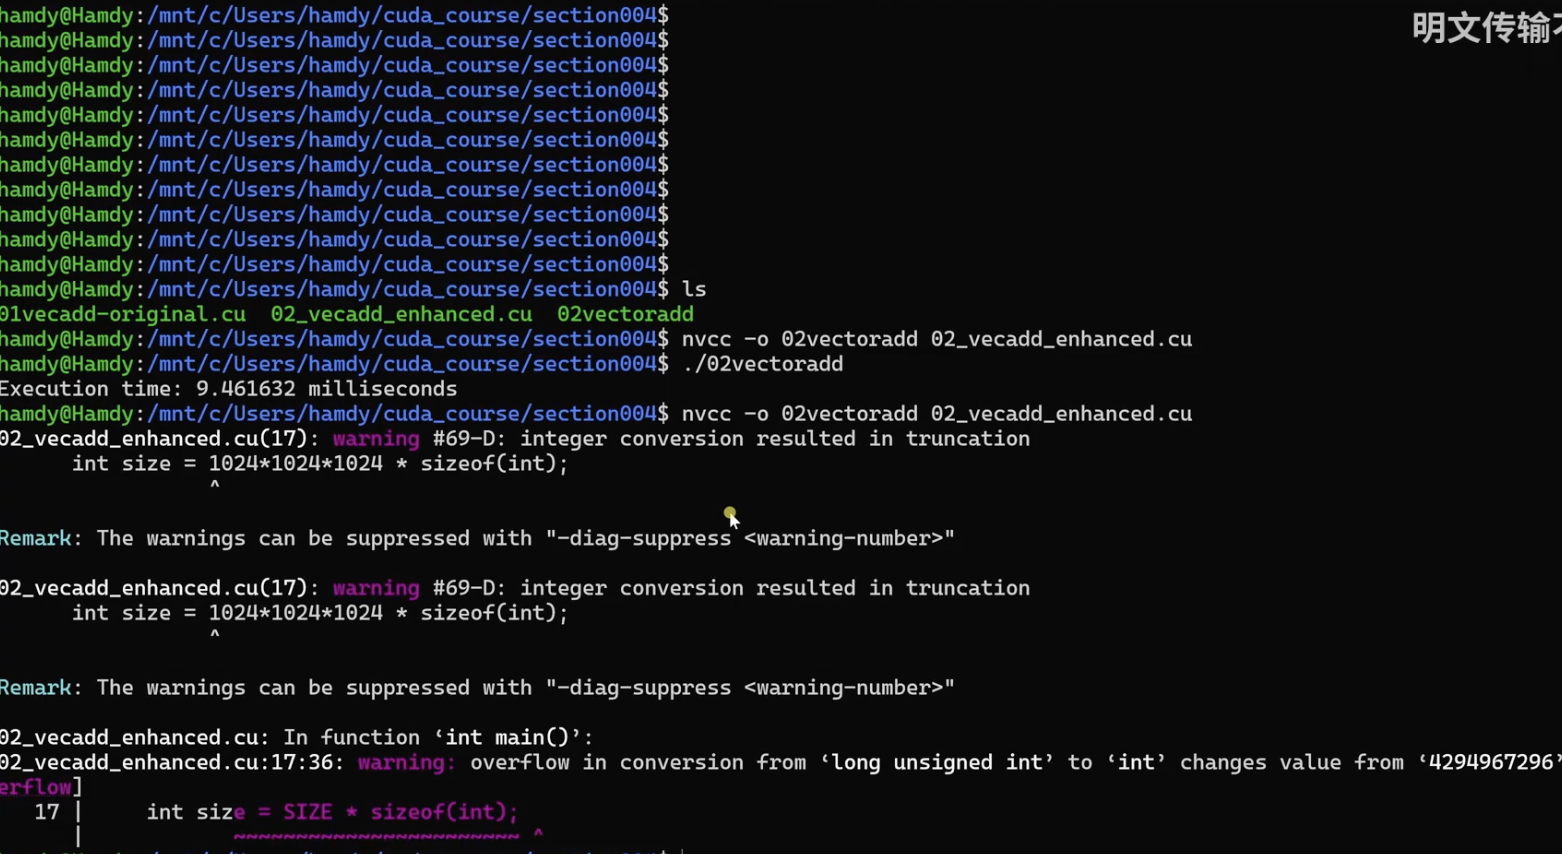
\includegraphics[width=0.75\linewidth]{resources/cuda-100.png}
    \caption{}
    \label{fig:placeholder}
\end{figure}

然而异步类型不同，因为异步类型在这里有 CUDA 启动函数代表，不会阻塞主机端或 CPU 执行下一条指令。这就是为什么如果不在这里放一个 \texttt{cudaDeviceSynchronize} 函数，执行 \texttt{cudaMemcpy}，可能会在执行完成之前复制结果。因为编译器不会停在这里，编译器将启动 GPU 核函数，然后进入下一条指令，这与在 \texttt{cudaMalloc} 函数中发生的情况不同。这就是为什么有不同的方法来检查异步操作的错误。这样做的方式就是使用一个叫做 \texttt{cudaGetLastError} 的函数。需要写一些像那样的东西，复制并把它放在这里。如所示，并不直接来到 GPU 任务本身写 \texttt{error = CUDA 函数} 或 \texttt{CUDA 启动}，不像之前做的那样。为什么？因为编译器不会停在这里，直到这个函数完成并返回一个错误存储在这里，它不会停在这里。这就是为什么不需要存储核函数执行的输出。相反，使用 \texttt{cudaGetLastError} 这个 CUDA Runtime API 函数。需要获取最后一个错误，它将存储在内存中的某个地方。而这个错误应该是 GPU 执行的最后一个函数的错误，在这种情况下就是向量加法函数。有两种不同的方法来处理这两类错误。同步错误，使用上面的方法；异步错误，使用 \texttt{cudaGetLastError} 方法。

\subsection{错误检查宏封装}

\begin{figure}
    \centering
    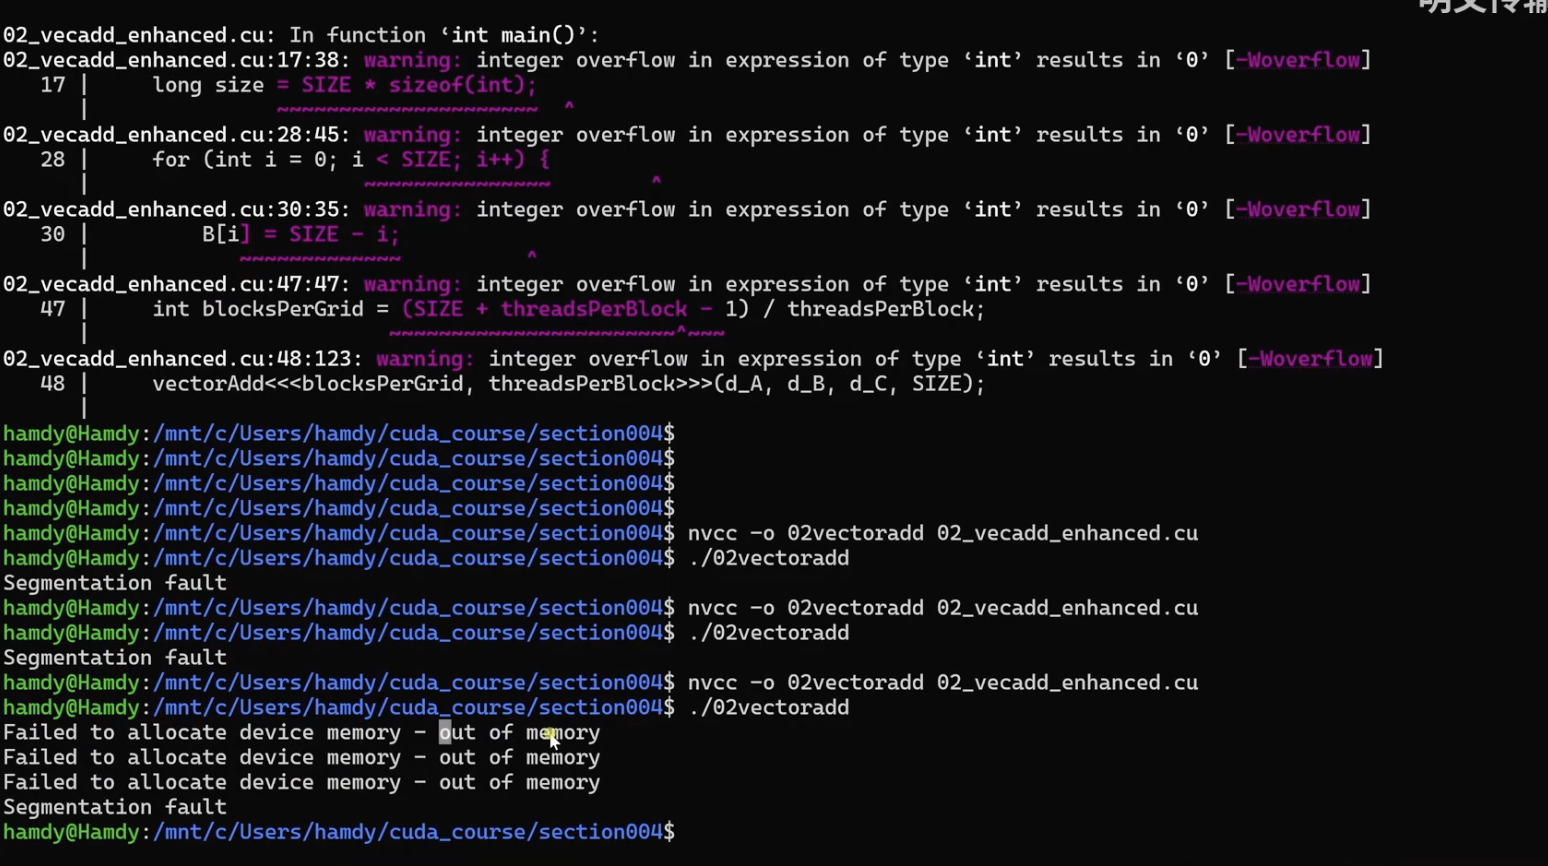
\includegraphics[width=0.75\linewidth]{resources/cuda-101.png}
    \caption{}
    \label{fig:placeholder}
\end{figure}

这里提一下，这三条指令在代码中重复了很多次。如所示，这里有这三条指令，这里也是同样的三条指令，这里也有。如果对所有 CUDA 函数使用错误检查，应该会看到它们在 \texttt{cudaMemcpy} 这里这两条函数以及 \texttt{cudaEventRecord}、用于输出的 \texttt{cudaMemcpy} 等等。这三条指令将在应用程序中重复多次，而没有必要。可以复制这部分，展示如何做到这一点。需要把这三条指令放在一个宏或一个函数里，然后在需要的时候调用它。如所示，有几行中有两个部分。第一部分是定义一个名为 \texttt{CUDA\_CHECK\_ERROR} 的宏。这个宏调用了一个名为 \texttt{cudaAssert} 的函数。\texttt{cudaAssert} 是一个函数，如所示，它接收一个来自 CUDA Runtime API 函数的错误作为输入，接收执行一个 CUDA 函数后返回的错误，然后检查错误是成功还是失败。如果成功，那么什么都不做。如果不成功，如所示，需要打印错误。但如果看这里的第一个关键字，会发现它叫做 \texttt{inline}。\texttt{inline} 指的是将这些指令内联到另一个代码中。这里不是一个分支，不是另一个函数，只是组织一下。需要复制 \texttt{CUDA\_CHECK\_ERROR}，并把它放在需要的地方。每当看到 \texttt{CUDA\_CHECK\_ERROR} 时，就是在调用 \texttt{cudaAssert}。而当调用 \texttt{cudaAssert} 时，并不是在执行另一个函数，只是复制这些指令，并把它们放在看到 \texttt{CUDA\_CHECK\_ERROR} 的任何地方。

编译并运行。不打算对所有函数都这样做，只是做一个示例。现在会看到区别，编译器正在尝试为第一个向量分配空间。看输出。如所示，看到一个叫做"GPUAssert: Out of memory"的输出，这发生在第 37 行。这就是在输出中看到的 GPUAssert。有 \texttt{\%s}，它对应错误本身，这就是为什么这里有错误本身，也就是内存不足分配。然后有文件名，也就是 \texttt{02\_enhanced\_vector.cu}。然后有行号，也就是 37。去看看 37 行，正确。但是为什么在这种情况下，没有看到三次向量 B 和向量 C 的失败？只看到向量 A 失败。因为如果看这里的 \texttt{cudaAssert}，会看到使用了 \texttt{exit}。这是因为如果无法为向量 A 分配空间，在没有足够空间的情况下，为什么要继续执行过程呢？需要退出，不需要执行那些不能正常工作的东西。在后续项目中，将使用这种错误检查方法，但不会再解释。这就是为什么需要按顺序观看所有章节。因为在每个章节中，都建立在之前解释的内容之上。

可以为异步操作做同样的事。复制这部分，来到这里。这是用于同步 CUDA 操作的，这是用于异步 CUDA 操作的。可以注意到区别，这里的 \texttt{cudaGetLastError} 函数在同步类别中没有。需要复制宏和 \texttt{cudaKernelAssert} 的定义。复制宏名，然后到这里用于核函数启动，但不需要写类似于 \texttt{error = 某物} 的东西，因为编译器不会停在这里。在完成之后，需要写一些类似那样的东西。在编译之前，把这个值减小到比如 32，以确保它在没有任何问题的情况下运行。现在执行完成没有任何问题。

以上就是关于错误检查的全部内容。通过本章的内容，应该理解了错误检查的重要性，以及如何将其用于不同的代码函数。在后续项目中，将使用错误检查而不再进行解释。
